\section{Linearisierung \skript{76}}
	\begin{minipage}[c]{10cm}
		\subsection{LTI-Systeme \skript{76}}
			\renewcommand{\arraystretch}{1.5}
			\begin{tabular}{|l|l|}
				\hline
				\textbf{Linearität} & \textbf{Zeitinvarianz}\\
				\hline
				$\Phi(x1+x2)=\Phi(x1)+\Phi(x2)$ & $\Phi(x(t-t_0)=\Phi(x)\cdot x(t-t_0)$ \\
				$\Phi(c\cdot x)=c\cdot \Phi(x)$ & \\
				\hline    
			\end{tabular}
			\renewcommand{\arraystretch}{1}
		\end{minipage}
		\begin{minipage}[c]{6cm}
			\subsection{Linearitätstest \skript{80}}
			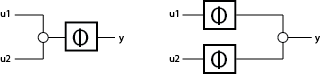
\includegraphics[width=6cm]{bilder/linearitaetstest}
		\end{minipage} \\
		
%	\begin{minipage}[c]{8cm}
%			\textbf{Lineare Operationen} \\
%			- Addition \\
%			- Integration \\
%			- Differentiation \\
%			daraus folgt, dass folgende Glieder auch linear sind: \\
%			- P-Glied \\
%			- I-Glied \\
%			- PT1-Glied
%	\end{minipage}
		


	\subsection{Linearität in den Parametern}
		Eine Funktion $f$ ist linear in den Parametern, wenn sie durch eine Linearkombination der Parameter geschrieben werden kann. Die Funktionen in $t$ müssen dabei nicht linear sein: \\
		$f(t) = \sum\limits_{j=1}^m a_j \cdot f_j(t)$ \\
		Beispiel: $y = \left[\begin{matrix} t^2 & sin(t) \end{matrix} \right] \cdot \left[\begin{matrix} a_1 \\ a_2 \end{matrix}\right]$ ist linear in den Parametern $a$
		
	
	
	\subsection{Einfluss der Lage einer Nichtlinearität}
		\begin{enumerate}
			\item	nicht lineare Blöcke dürfen \underline{nicht} vertauscht werden!\\			
			\item vertauschen von linearen Blöcken erlaubt falls ...\\
								... Anfangsbedingung = 0\\
								... interne Signale keine Rolle spielen
		\end{enumerate}
	  	
	\subsection{Erwünschte Nichtlinearität \skript{83}}
		In einem Prozess sind Linearitäten meist erwünscht, da sie meist mit
		Gleichungen zu lösen sind.
		Viele Efekte, wie zum Beispiel die Modulation oder so sind aber gerade erst
		durch Nichtlinearitäten möglich. Daher unterscheidet man:\\
	\begin{minipage}[c]{8cm}
		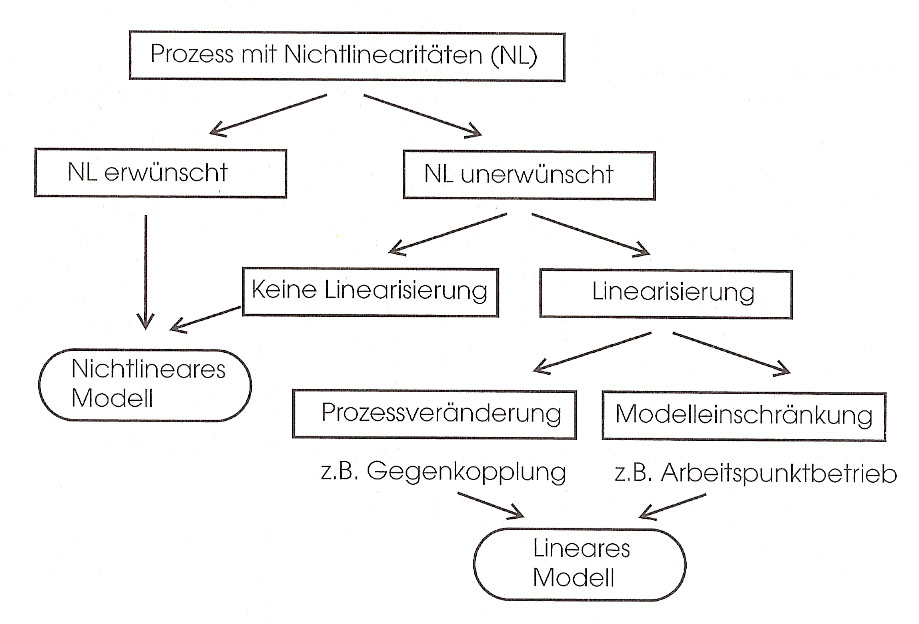
\includegraphics[width=8cm]{./bilder/Liste_Nichtlinearitaeten.jpg}
	\end{minipage}

		

\newpage
	
\subsection{Erfassen von nicht linearen Kurven}
	\subsubsection{Messung einer statischen Kennlinie \skript{85}}
	\begin{minipage}{10cm}
		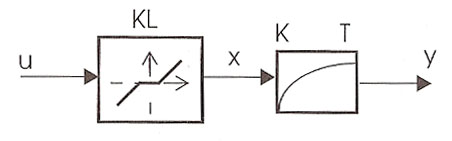
\includegraphics[width=6cm]{./bilder/NichtlinearMitPT1.jpg}   
    \end{minipage}
	\begin{minipage}{7cm}
    	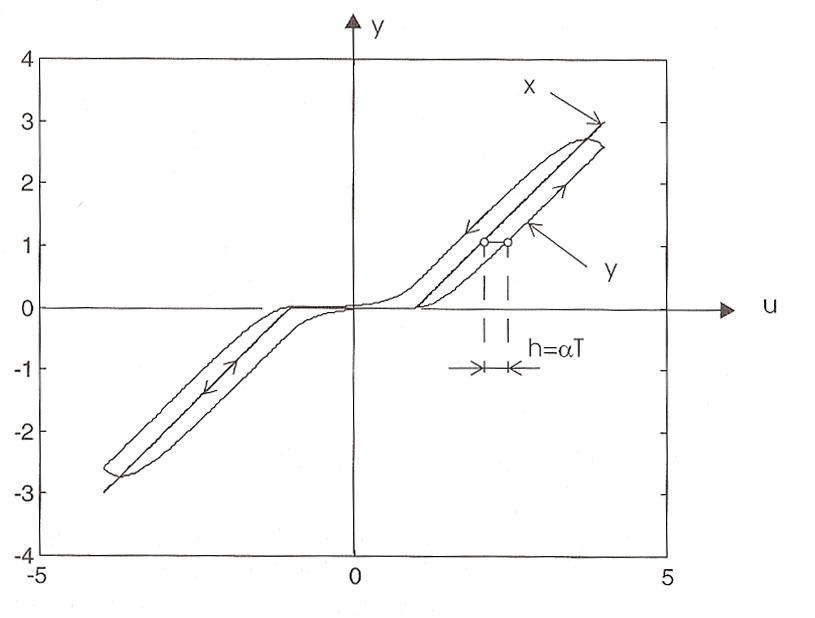
\includegraphics[width=4.5cm]{./bilder/NichtlinearMitPT1_dia.jpg}
    \end{minipage}\\
		\begin{tabular}{p{4cm}  p{14cm}}
				\textbf{statische Messung:} &
				schrittweises anlegen eines konstanten Signalwertes (Treppenfunktion)
				am Eingang. Dabei muss jedes mal der Einschwingvorgang abgewartet werden.\\
				
				\textbf{dynamische Messung:} &
				Am Eingang wird eine Dreieckspannung angelegt. Eine zu hohe Rampensteilheit
				führt zu einer ``unechten Hysterese`` die als physikalische Eigenschaft gar
				nicht existiert.\\
		
				$h = \alpha \cdot T$ & $h$: Hysteresenbreite\\
				\parbox{4cm}{falls $h$ von $\alpha$ abhängt ist die Hysterese unecht} & $\alpha$: Rampensteilheit $[1/s]$\\
				& $T$: Zeitkonstante des PT$_1$\\
				& 
			
		\end{tabular}


	\subsubsection{Mathematische Erfassung einer Messkurve \skript{88}}
	\begin{floatingfigure}[r]{12cm}
    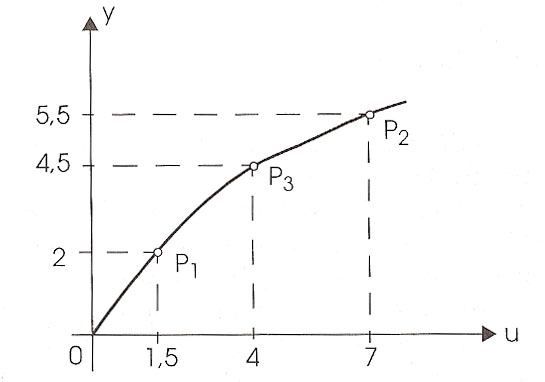
\includegraphics[width=10cm,height=3cm]{./bilder/KennlinieMitStuetzwerten.jpg}
	\end{floatingfigure}
   	
     	\begin{enumerate}
     	\item \textbf{Wahl einer geeigneten Funktion:}\\
     	Gesucht ist ein Graph, der eine ähnliche Form
		hat wie die Messkurve. Günstig sind Polynome, da sie mathematisch einfach zum
		beschreiben sind, aber auch Sinus- oder Arctan- Funktionen	\\ 
     	
        \item \textbf{Bestimmung der Parameter:}
          \begin{enumerate}
           \item Methode der ausgewählten Punkte (für GL nicht linear in Paramater):\\
          		\begin{enumerate}
                    \item Gleich viele Messpunkte wie frei zu wählende Parameter der
           			Approximationsfunktionen.
           			\item Einsetzen der Koordinaten der Messpunkte in die Gleichungen.
           		\end{enumerate}
           	\item Methode der kleinsten Fehlerquadrate (für GL linear in Parameter):
           		\begin{enumerate}
                     \item Mindestens gleich viele Messpunkte wie Parameter der
           		Appxomationsfunktion, können jedoch mehr gewählt werden. z.B. \\
						Näherungsfunktion: $y = ax^2 + bx$ \\
						P1:		$2.0 = a\cdot 1.5^2+b\cdot 1.5$ \\
						P2: 	$5.5 = a\cdot 7^2+b\cdot 7$\\
						P3: 	$4.5 = a\cdot 4^2+b\cdot 4$         		
           		\item Fehler bilden zwischen Messpunkt und Funktionspunkt. z.B.\\
           		\begin{minipage}{10cm}
           				P1:  	$e_1=2-y=2-(a(1.5)+b(1.5)^2)$\\
           				P2:  	$e_2=5.5-y=5.5-(a(7)+b(7)^2)$\\
           				P3:  	$e_3=4.5-y=4.5-(a(4)+b(4)^2)$\\
           		\end{minipage}
				\begin{minipage}{6cm}
					\textbf{Matrixschreibweise:}\\
						$\left[\begin{matrix}
						2.0 \\5.5\\ 4.5
						\end{matrix}\right] =
						\left[\begin{matrix}
						1.5^2 & 1.5 \\ 7^2 & 7\\ 4^2 & 4
						\end{matrix}\right] \cdot
						\left[\begin{matrix}
						a \\ b
						\end{matrix}\right] \Rightarrow
						\vec{y} = M \cdot \vec{p}$
				\end{minipage}\\           		
           		\item Nach Gauss ist die beste Näherung, wenn die Summe der
           		Fehlerquadrate minimal wird. \\
           		\begin{minipage}{8cm}
           			$\Longrightarrow$ S =$ e_1^2+e_2^2+e_3^2=min$\\
           			$\frac{\delta S}{\delta a}=
           			2 e_1 \frac{\delta e_1}{\delta a}+
           			2 e_2 \frac{\delta e_2}{\delta a}+
           			2 e_3 \frac{\delta e_3}{\delta a}=0$\\
           			$\frac{\delta S}{\delta b}=
           			2 e_1 \frac{\delta e_1}{\delta b}+
           			2 e_2 \frac{\delta e_2}{\delta b}+
           			2 e_3 \frac{\delta e_3}{\delta b}=0$\\
           		\end{minipage}
				\begin{minipage}{9cm}
					\textbf{mit Matrizen:}\\
						$M$ nicht überbestimmt: $\vec{p} = M\backslash\vec{y} = M^{-1} \cdot \vec{y} \rightarrow$ \\
						$M$ überbestimmt: $\vec{p} = pinv(M)\cdot \vec{y} = (M^TM)^{-1}M^T \cdot \vec{y}$\\
				\end{minipage}           		
           		\item Nachteil dieser Methode ist, dass es meist einen grossen
           		Rechenaufwand ergibt. Sie ist jedoch genauer als die erste Methode.
           		Ausserdem geht die Approixmationsfunktion nicht durch die Messwerte.
           		\end{enumerate}
		\end{enumerate}
	\end{enumerate}
	
\newpage

	\subsection{Linearisierung}
		\subsubsection{Modelleinschränkung \skript{93}}
			Praktisch alle physikalische Systeme unterliegen gewissen Aussteuergrenzen.
			In diesen können sie linear sein. Es muss darauf achten, dass  das System
			diese nicht überschreitet. \\
			z.B. Festwert-Regelung: Die Kennlinie wird nur beim Einschalten durchlaufen.
			Ab dann bewegt sich die Regelung nur in einem sehr kleinen Bereich um den
			Arbeitspunkt, wo die Kennlinie linearisiert werden kann. \\
			
		\subsubsection{Arbeitspunkt \skript{94}}
			Wenn eine Kennlinie für einen bestimmten Aussteuerung einen nicht zu grosse
			Krümmung hat, kann man in der Näherung diese durch die Tangente ersetzen, und
			somit wieder linear rechnen. \\
			Trigonometrische Funktionen bei Arbeitspunkt $\alpha = 0$: $\qquad \sin \alpha \approx
			\alpha \qquad \tan \alpha \approx \alpha \qquad \cos \alpha \approx 1$ \\
			\textbf{Vorgehen} \\
			\begin{minipage}[c]{5cm}
				\includegraphics[width=5cm]{bilder/LinArbeitspunkt}
			\end{minipage}
			\begin{minipage}[c]{16cm}
				\begin{enumerate}
					\item DGL der nichtlinearen Regelstrecke bestimmen
					\item Alle Signale so formulieren: $x = x_0 + \Delta x,$ z.B. $v=v_0 + \Delta v$ (Arbeitspunkt + Abweichung)
					\item Beziehung zwischen den Arbeitspunkt-Werten der verschiedenen Signale aufstellen.
					\item DGL mit $\Delta x$ angeben.
					\item Vernachlässigen der Termen höherer Ordnung, z.B. $\Delta x^2$
				\end{enumerate}
	
			\end{minipage}
			
			\textbf{Beispiel:}\\
			\begin{tabular}{lll}
				DGL: & $v=\int(F_s - K\cdot v^2) \cdot \frac{1}{m} dt \Leftrightarrow Kv^2 + m\dot{v} = F_s$ &\\
				$x = x_0 +\Delta x$: & $v(t) = v_0 + \Delta v$ & $v_0$ vorgegeben \\
				& $F_s(t) = F_{s0} + \Delta F_s$ & $F_{s0} = K\cdot v_0^2$ \\
				DGL mit $\Delta x$: & $v(t) = \int\frac{1}{m}(F_s(t) - K \cdot v(t)^2) dt$ & \\
				& $\Leftrightarrow v_0+\Delta v = \int\frac{1}{m}(F_{s0}+\Delta F_s - K(v_0+\Delta v)^2 dt$ & \\
				& $\Leftrightarrow v_0+\Delta v = \int\frac{1}{m}(Kv_0^2+\Delta F_s - K(v_0^2+2v_0\Delta v+\Delta v^2) dt$ & \\
				$\Delta x^2$ vernachlässigen: & $\Leftrightarrow v_0+\Delta v = \int\frac{1}{m}(Kv_0^2+\Delta F_s - K(v_0^2+2v_0\Delta v) dt$ & \\
				Umformen: & $m\Delta\dot{v}+2Kv_0\Delta v = \Delta F_s \Rightarrow m\Delta\dot{v}+K_0\Delta v = \Delta F_s$ & mit $K_0 = 2Kv_0$ \\
			
			\end{tabular}

		\subsubsection{Durch inverse Kennlinie \skript{95}}
		\begin{minipage}{11cm}
			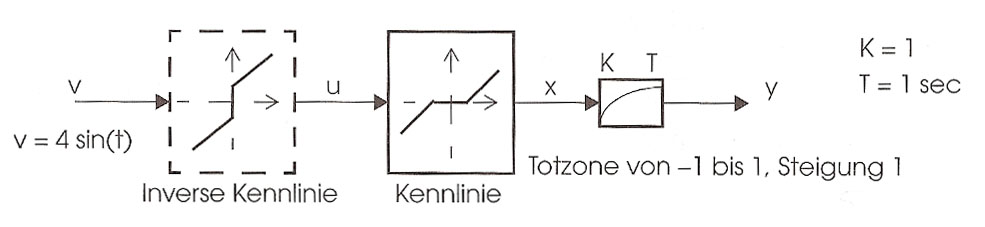
\includegraphics[width=10cm]{./bilder/Kennlinienkompensation.jpg}
        \end{minipage}
		\begin{minipage}{6cm}
        	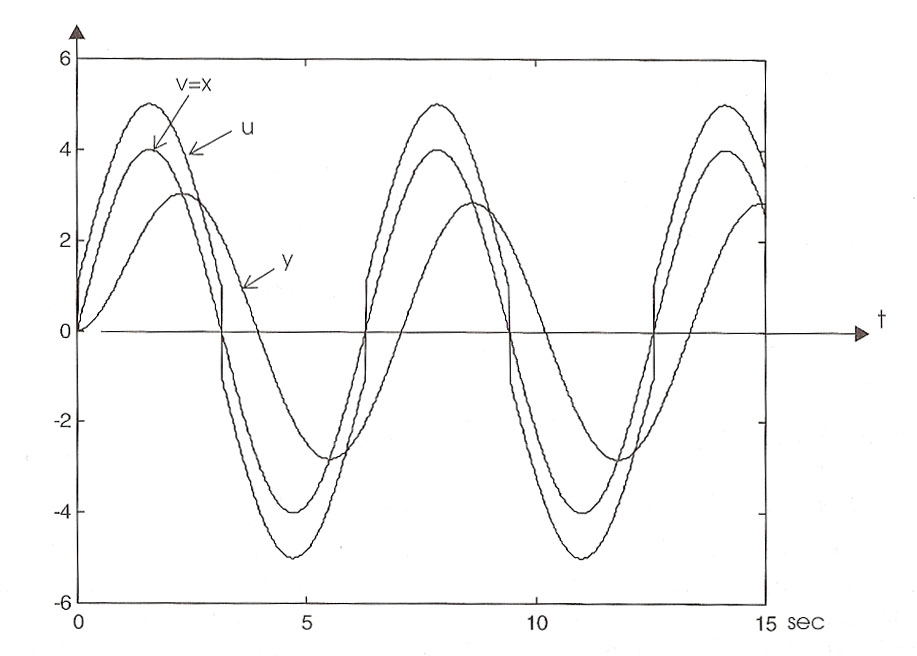
\includegraphics[width=4cm]{./bilder/Kennlinienkompensation_dia.jpg}
        \end{minipage}\\
			Durch das Vorschalten der Inversen Kennlinie kann man die Nichtlinearitäten
			beheben. Das System als ganzes reagiert nun linear, das Innere des System
			jedoch immer noch nicht, wie man an den Kennlinien gut erkennen kann.
		\subsubsection{Durch Gegenkopplung \skript{96}}
				\begin{minipage}{11cm}
			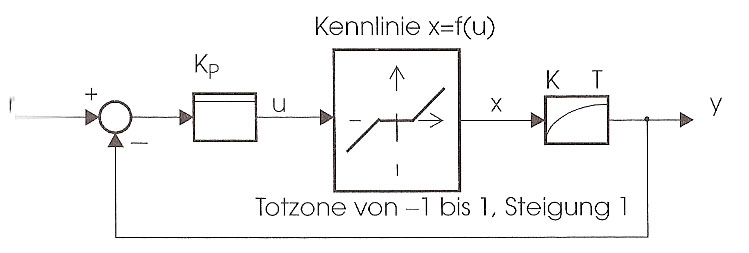
\includegraphics[width=8cm]{./bilder/Gegenkopplung.jpg}
        \end{minipage}
		\begin{minipage}{9cm}
        	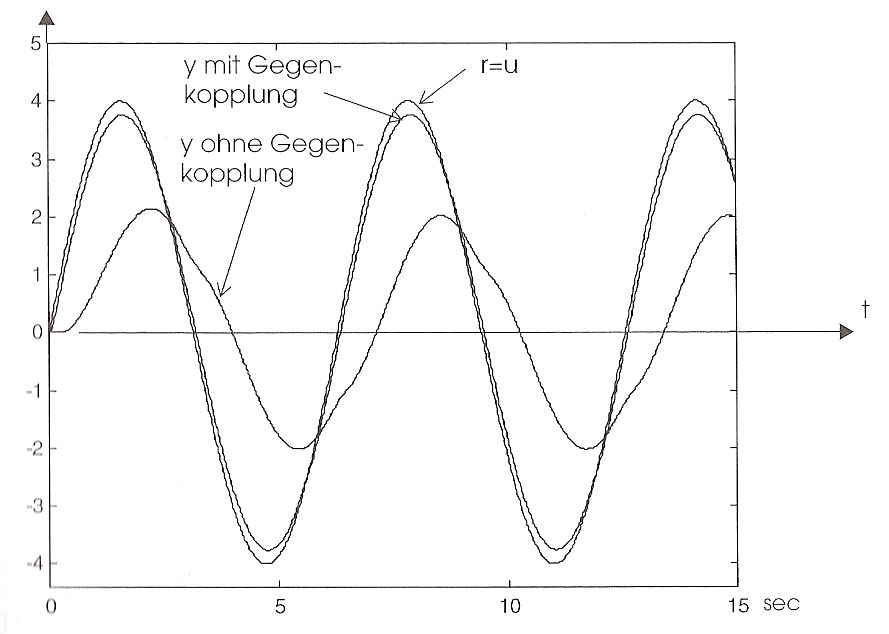
\includegraphics[width=4cm]{./bilder/Gegenkopplung_dia.jpg}
        \end{minipage}\\
			Da ein Prozess variierende Koefizienten besizten kann, kann die Kompensation
			nicht immer mit der inversen Kennlinie geschehen. Deshalb ist es oft
			günstiger die Nichtliniearitäten mit einer Gegenkopplung zu kompensieren.
			Diese ist umso wirksamer je grösser die Verstärkung $K_p$ ist.
			Es können jedoch Stabilitätsprobleme auftreten.
			

			
